{希尔排序是{对直接插入排序进行改进后提出来的,又称缩小增量排序}。其基本思想是:不断地把待排序的一组记录按间隔值分成若干小组,分别进行组内直接插入排序,这个规则就是增量。举例如下。}{}

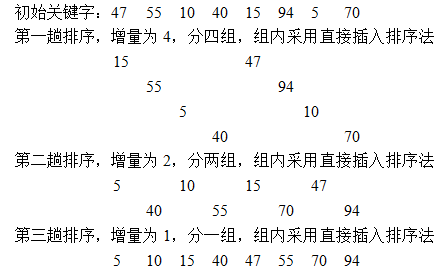
\includegraphics[width=3.70833in,height=2.30208in]{png-jpeg-pics/194B080AB7E87FA66145FF709D9D6B1B.png}

{\textbf{算法分析:}}{希尔排序速度一般要比直接插入排序快。希尔排序的平均时间复杂度为O(nlog}\textsubscript{2}{n)。希尔排序是}\textbf{不稳定}{的排序方法(即相同值的元素,排序前后的顺序发生变化了)。}
